
\subsection{Performance Prediction Data Set}

{\bfseries RQ3} asks if the aforementioned method can be expanded to other kinds of data. To answer this, we have used the performance prediction data set collected by Siegmund et al. for their ICSE '12 paper~\cite{sven12}. The data sets have been deployed as a part of the \textsc{SPLConqueror} tool\footnote{\url{fosd.de/SPLConqueror}}. This data set contains six examples of real world configurable systems that cover a broad spectrum of scenarios, see figure \ref{fig:cpm} for a summary. The systems have different characteristics (lines of code: 40 thousand to 300 thousand; Valid configurations: 192 to about 3.9 million), different implementation languages (C, C++, and Java), different mechanism (conditional compilation, configuration files, and command-line options), and different domains (Web servers, compilers, encoders, and databases). The data contains a measurement of all the configurations that are invoked by the benchmarking tool. The measurements were conducted 5 to 20 times and the mean of all measurements for each configuration was recoded.

For our experiments, we randomly split the data sets into two equal halves, one for training and the other for testing. The planning phase learns configuration settings from the training half and plans for changes in the test half aiming to optimize the performance of the test instances. We repeat our measurements 20 to 25 times to overcome measurement bias.
\section{Experimental Design}

\subsection{The Rig}

The experimental rig for defect prediction is shown in Figure \ref{fig:rig}. It works as follows: 
\bi
\item We use an {oracle} (Random Forest + SMOTE) to determine whether a certain test case is defective or not. 
\item If the oracle suggests that an instance is defective, then we use HERE to apply the recommendations to that test instance. 
\item The oracle is then used to predict the attributes in the modified instance.
\item The statistical significance of the changes are verified using the cliffs delta measure described below.
\ei

For run time optimization, we use a similar rig. The oracle is Random Forest, and it predicts for run times of specific configuration. HERE is used to generate a recommended configuration to reduce the run times. The run time is measured by the oracle. The reduction of run times are expressed as fractions of the original (also referred to as baseline) run time.

Note that we report the performance scores as a comparison between the oracle's prediction \textit{before} and that \textit{after}. We refrain from using the \textit{actual} defects in the data sets to perform the same comparison. This is because the oracle is limited in its ability to predict defects, there are instances that are inherently misclassified. These misclassifications however are not affected by the planner. Therefore, by comparing the defect counts before and after applying the planner and doing so with a the same oracle would give us an accurate albeit relativistic measure of performance.


In should be noted  that the standard 10-way cross-validation
procedure used  in data mining does not necessarily demonstrate G-causality.  In a N-way cross-val experiments, the data is divided into $N$ bins.  
$N-1$ bins are used for learning and the results are tested
on the  remaining bin.
This is repeated $N$ times, each time using a different bin for the test set.
This approach can not be used to demonstrate causality since, if the initial data is collected
over (say) $N$ months, then it is possible that the test set contains observations collected
{\em before}   items seen in the training set. 

Jiang et al.~\cite{me11f} and Lumpe et al.~\cite{me11f} propose a modification to cross-validation.
which lets a researcher
demonstrate G-causal defect effects in software engineering.
In this modification, we  divide project data  into $N$ bins, each of with contain data collected at similar t

imes.
They then sort those bins (on the collection date) and use bins $i,j$ to build models that
are applied to bin  $k$ where 
$i<j<k$. Note that this procedure ensures that we are building theories on data seen
before the test data.

We adapt the work of Jiang,Lumpe et al.  as follows.


blah blah data. algorithms. statistics

\section{Releated Work}

Our prior work in generating policies relied upon a Monte Carlo
analysis of an underlying model~\cite{me07f}. This approach had three major problems.
Firstly, enough domain knowledge had to be collected to build that model
and this can take a long time. For example, in our previous work we used three software process models from
the Unviersity of Southern California that were initially
developed and updated for nearly two decades from 1981~\cite{boehm81} to 2000~\cite{boehm00b}.

Secondly, there is the computational cost of running those models.
While 

~\cite{}-- which suffered from the problem of (a)~the effort required to collect the domain knowledge to build
problem in certifying the underlying model;
 (b)~the computational problem of running that model enough
times to learn patterns in that data; and (c)~ requrearea used large scale simulations or large


While
our case studies are defect and runtime reduction, HERE is a general
purpose algorithm that could be applied to any table of data with at least
one column whose values can be sorted from ``desired'' to ``undesired''.



{\bf RQ1: Can Instance-based Learning techniques be used to create Planning tools that can better analyse software defect?} 


{\bf RQ2: Can lessons learnt from local policy generators be useful for generating solutions that can be used to mitigate defects in software systems?} 

{\bf RQ3: Can such instance-based planners be applied to other software engineering paradigms?}
We check if the proposed instance-based planner is applicable to performance prediction.

\section{Motivating Example}
\section{Background}
\section{Instance Based Learning}

Assessing the quality of solutions to a real-world problem can be extremely hard~\cite{menzies2005xomo}. In several software engineering applications, researchers have models that can emulate the problem, for instance there is the COCOMO effort model~\cite[p29-57]{boehm2009software}, the COQUALMO defect model~\cite[p254-268]{boehm2009software}, Madachy’s schedule risk model~\cite[p284-291]{boehm2009software}, to name a few. Using these models it is possible to examine several scenarios in a short period of time, and this can be done in a reproducible manner. However, models aren't always the solution, as we shall see. 

There exist several problems where models are hard to obtain, or the input and output are related by complex connections that simply cannot be modeled in a reliable manner, or generation of reliable models take prohibitively long ~\cite{Ludewig2003}. Software defect prediction is an excellent example of such a case. Models that incorporate all the intricate issues that may lead defects in a product is extremely hard to come by. Moreover, it has been shown that models for different regions within the same data can have very different properties \cite{localvsglobal}. This makes it extremely hard for one to design planning systems that are capable of mitigating these defects.

An alternative approach would be to make use of an instance based approach, an example of case based reasoning strategy, in place of the conventional model based approach. Instance based approaches have been used extensively by the effort estimation community, see~\cite{keung2008analogy, 6600685, walkerden1999empirical, shepperd1997estimating, kocaguneli2010use}. 

This approach has been proposed as an alternative to closed form mathematical models or other modeling methods such as regression \cite{keung2008analogy}. There are several other reasons for instance based approaches being a useful tool, see~\cite{6600685}. As pointed out by~\cite{walkerden1999empirical} it can be used with partial knowledge of the target project at an early stage which could be a very useful tool in preventing software defects. Instance based approaches are also rather robust in handling cases with sparse samples \cite{1438374}. All these features are desirable and suggest that instance-based approach is a useful adjunct to traditional model based approach. 

In this paper the instance based learning principle is used to first cluster the training data and then create contours in the data. These contours can then be used by test cases to infer meaningful information in order to improve it. The entire process is described in greater detail in the following sections. We would like to stress that the purpose of our work is not to promote instance-based planning over model based analytics, rather it is to suggest an alternative when model based approaches cannot be used.

\subsection{Spectral Learning using WHERE}
The algorithm uses WHERE to recursively cluster the input data to identify subsets in the training data that a test instance can learn from. WHERE is a spectral learner which uses the FastMap heuristic to estimate the first principal component. It then recursively partitions the data into two halves along the Median point of the projection on the first principal component, terminating when a half has less than $\sqrt{N}$ items.   

\subsection{Planning changes using HERE}
We propose the HERE algorithm as a tool to plan changes in the original test data. Figure~\ref{fig:what} highlights the procedure by which HERE operates. It begins by creating clusters which are generated using the WHERE algorithm discussed above. Following this, a nearest neighbour scheme is applied to identify pairs of nearby clusters. A contour is constructed with these clusters at the vertices to characterize the cluster pairs.

The mutation policy works by projecting the test instance onto the contours and identifying the the contour on which the test instance has the largest scalar projection. The planner then reflects over the vertices of the chosen contour, identifying the \textit{better} vertex among the two. Now, a new instance is generated by \textit{mutating the attributes} of the test instance towards the better vertex and away from the worse vertex. This process is repeated for all the test instances that are considered defective by the defect prediction scheme, discussed below.

\subsection{Feature Weighting} \label{fwt}
The algorithm also allows for a feature weighting and pruning scheme. We have employed a simple (and fast) attribute ranking method where the features are sorted based on their ability to find meaningful splits in the dependent class of the data, see ~\cite{hall03}. Features that can find splits with the \textit{lesser variance} in the dependent variable are \textit{ranked higher} than features that don't. 

We reason that the most informative feature must undergo a larger change as compared to other features. Therefore, when feature weighting is employed, the higher ranked features are mutated by a larger extent. Additionally, we have also included information pruning. Here we mutate only the top X\% of the features in each test instance. The remaining features remain unaltered. 

\begin{figure}
\centering
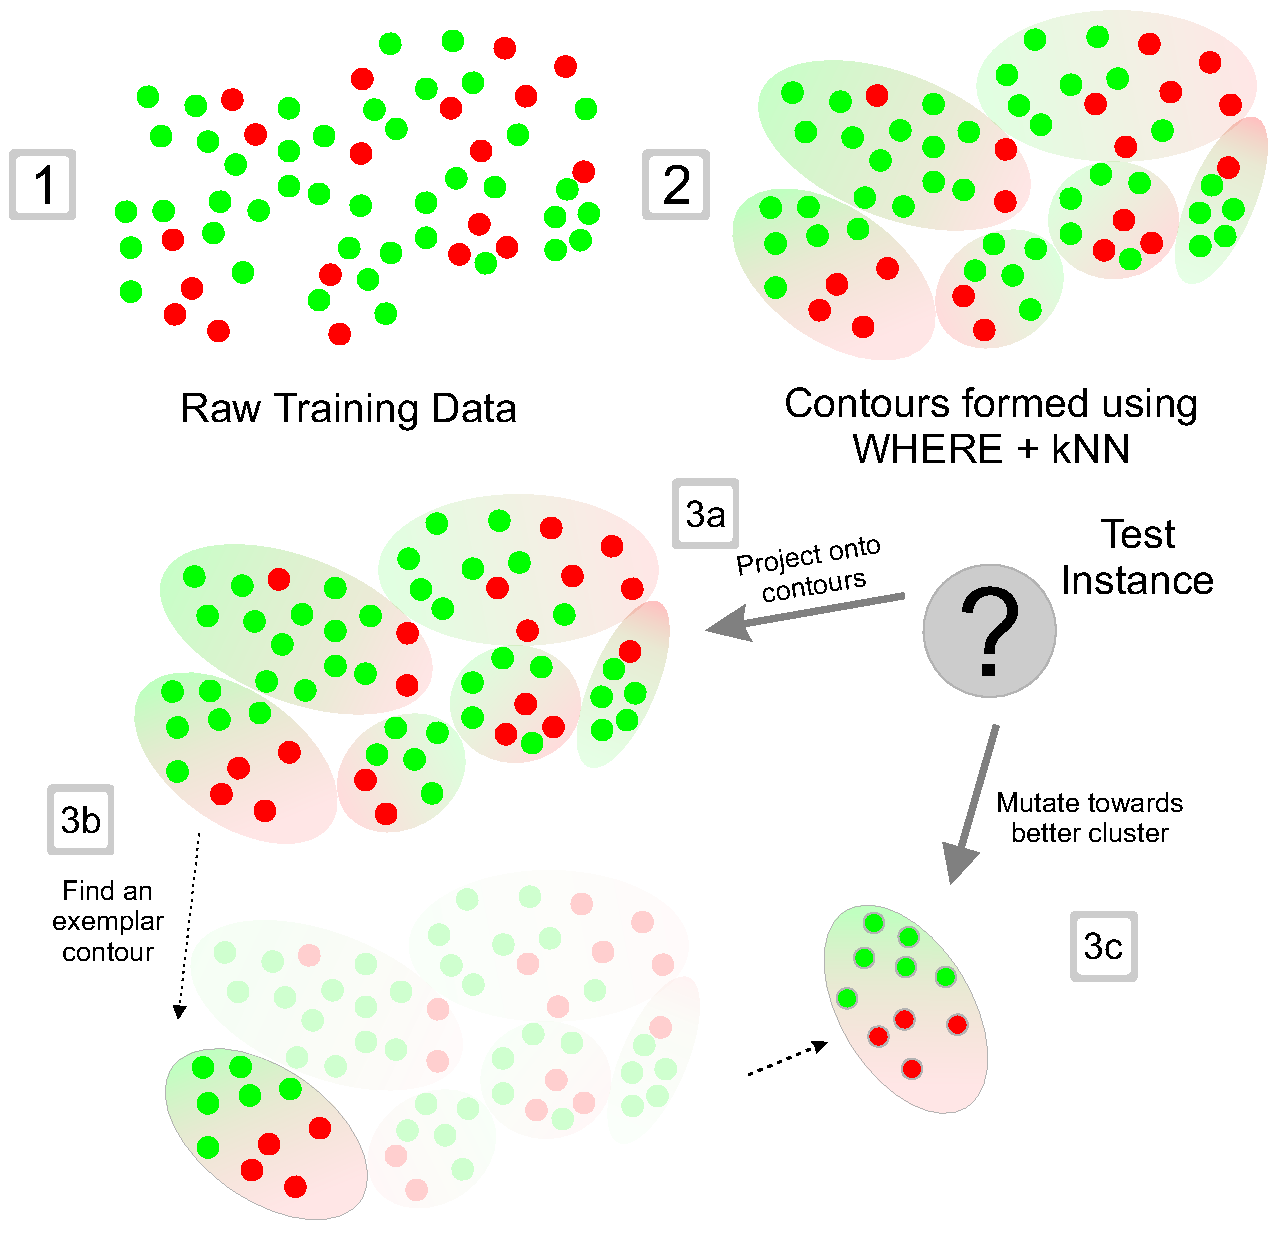
\includegraphics[width=\linewidth]{_figs/WHAT-Clusters2.pdf}
\caption{HERE}
\label{fig:whatflow}
\end{figure}



\subsection{Defect Prediction}

To validate the treatments that have been suggested by our planner, we need to have defect predictors that capable of identifying if a certain module may (or may not) have a defect. A recent IEEE TSE paper by Lessmann et al.~\cite{lessmann} compared 21 different learners for software defect prediction: 
\bi
\item
{\em Statistical classifiers:}
Linear    discrimin analysis,
Quadratic discrimin analysis,
Logistic regression,
Naive Bayes,
Bayesian networks,
Least-angle regression,
Relevance vector machine,

\item
{\em Nearest neighbor methods:}
k-nearest neighbor,
K-Star

\item
{\em Neural networks:}
Multi-Layer Perceptron,
Radial bias functions,

\item
{\em Support vector machine-based classifiers:}
Support vector machine,
Lagrangian SVM
Least squares SVM,
Linear programming,
Voted perceptron,

\item
{\em Decision-tree approaches:}
C4.5,
CART,
Alternating DTs
\item
{\em Ensemble methods:}
\textbf{Random Forest},
Logistic Model Tree.
\ei

They concluded that Random Forrest was the best method, CART being the worst.

Random Forest is an ensemble learning scheme that constructs a number of decision trees at the training time, for a test instance it outputs the mode of the classes of individual tree. It's patent from how random forest operates that the prediction will suffer if there is an imbalance in classes during the training. Unfortunately, the data sets explored here do suffer from severe skewness, as highlighted in~\ref{fig:classimb}. A study conducted by Pelayo and Dick~\cite{smote2} inspected this issue. They showed that the SMOTE technique~\cite{smote} can be used to improve recognition of defect-prone modules. 

In short, SMOTE works by under-sampling the majority class and oversampling all the minority classes in the training data. We use a similar approach with one minor addition to the original algorithm. In our implementation of SMOTE we have introduced an additional step called \textit{resampling}, wherein we ensure that after we do the over/under sampling, the new training data does not have any of the original rows. The new training data merely resembles the original data. This is done as a precautionary measure, so as not to have HERE and Random Forest train on the same training data. 
%Its worth noting that both HERE and Random Forest require some data to train. In order to prevent the two from using the same data to train, we run SMOTE by  \textit{resampling} the classes. Re-sampling 


\section{Data sets}

The following section describes the experimental rig and the experiments used to measure the performance of HERE on 10 defect data sets and 6 performance prediction data sets.

\subsection{Defect Data Set}
The data was obtained from the PROMISE repository\footnote{Promise Repository: \url{openscience.us/repo}}. For the defect data we investigated 32 releases from 11 open source Java projects defined by the metrics highlighted in figure ~\ref{fig:ck}: \kw{Apache Ant} (1.5 -- 1.7), \kw{Apache Camel} (1.2 -- 1.6), \kw{Apache Ivy} (1.1 -- 2.0), \kw{JEdit} (4.1 -- 4.3), \kw{Apache Log4j} (1.0 -- 1.2), \kw{Apache Lucene} (2.0 -- 2.2), \kw{PBeans} (1.0 and 2.0), \kw{Apache POI} (2.0 -- 3.0), \kw{Apache Synapse} (1.0 -- 1.2), \kw{Apache Velocity} (1.4 -- 1.6), and \kw{Apache Xalan-Java} (2.5 -- 2.7). 

Given the empirical nature of the data, it is import to design an experiment such that the planning phase uses only the \kw{past} data to learn trends which can then be applied to the \kw{future} data. Thus for our experiment we use data sets that have at least two consecutive releases. 
\begin{itemize}
\item To generate recommendations for a release $i$, the planner uses releases releases $(i-1)$ and $(i-2)$.
\item The predictor also uses releases $(i-1)$ and $(i-2)$. However, we use SMOTE with re-sampling in order to handle the class imbalance in the data and to prevent the predictor from using the same training data as the planner.
\end{itemize}